\newpage
\section{Tests unitaires}

Le code présent ci-dessous est celui de la fonction qui permet de rajouter une nouvelle question au deck.
Différent cas de vérification ont lieu avant de permettre à une question quelconque d'être rajoutée.
Le premier cas sert à vérifier que l'objet en entrée ne soit pas null, si c'est le cas, alors la fonction renverra false.
Le deuxième consiste à vérifier que l'ajout ne cause pas de doublon, si c'est le cas, l'exception QuestionDoubleException sera appelée, et false sera renvoyé comme résultat.
Le troisième cas consiste à vérifier que le thème de la question correspond bien à celui de la carte, si c'est pas le cas, QuestionIncompatibleException sera appelée et false sera renvoyé comme résultat.
Le dernier cas de vérification consiste à vérifier qu'il n'y ait pas plus que le nombre maximal de question sur une carte, dans le cas de notre jeu ce dernier équivaut à 4.
Si une 5\up{ème} est rajoutée, l'exception BasicCardOverMaxQuestionsException sera appelée et le résultat sera false;
Si tous les cas de vérifications sont réussis, alors la fonction va ajouter la nouvelle question à la carte, et le résultat sera true.

\begin{lstlisting}
/**
 * Function used to add a new question to the card
 * 
 * @param q The question that the user wishes to add to his card
 * 
 * @return true if added, false if not
 */
public boolean add( Question q )
{
    try
    {
        if ( q == null )
        {
            throw new NullPointerException();
        }
        if ( questions.contains( q ) )
        {
            throw new QuestionDoubleException();
        }
        if ( q.getTheme() != theme || !q.getAuthor().equalsIgnoreCase( author )
                || !q.getSubject().equalsIgnoreCase( subject ) )
        {
            throw new QuestionIncompatibleException();
        }
        if ( questions.size() == 4 )
        {
            throw new BasicCardOverMaxQuestionsException();
        }
        return questions.add( q.clone() );
    }
    catch ( NullPointerException npe )
    {
        npe.printStackTrace();
        return false;
    }
    catch ( QuestionDoubleException qde )
    {
        qde.printStackTrace();
        return false;
    }
    catch ( QuestionIncompatibleException qie )
    {
        qie.printStackTrace();
        return false;
    }
    catch ( BasicCardOverMaxQuestionsException bcomqe )
    {
        bcomqe.printStackTrace();
        return false;
    }
}
\end{lstlisting}

Dans les tests unitaires, cette fonction est vérifiée en lui injectant les différents cas possibles.
Voici une partie du code des tests unitaires qui ont lieu sur BasicCard, ici on ne vérifie que les différentes interactions avec la fonction ``add'' et on s'assure que les différents cas de vérifications soient bien respéctés.

\begin{lstlisting}
public class BasicCardTests
{
    private static BasicCard c1, c2;
    private static Question q1, q2, q3, q4, q5, q6, q7, q8, q9, q10, q11, q12;

    @BeforeAll
    static void initAll()
    {
        c1 = new BasicCard( "Giorgio Caculli", Theme.INFORMATICS, "Acronyms" );
        c2 = c1.clone();
        q1 = new Question( "Giorgio Caculli", Theme.INFORMATICS, "Acronyms", "What does RAM stand for?",
                "Random Access Memory" );
        q2 = new Question( "Giorgio Caculli", Theme.INFORMATICS, "Acronyms", "What does JAR stand for?",
                "Java ARchive" );
        q3 = new Question( "Giorgio Caculli", Theme.INFORMATICS, "Acronyms", "What does WWW stand for?",
                "World Wide Web" );
        q4 = new Question( "Giorgio Caculli", Theme.INFORMATICS, "Acronyms", "What does CPU stand for?",
                "Central Processing Unit" );
        q5 = new Question( "Giorgio Caculli", Theme.INFORMATICS, "Acronyms", "What does GPU stand for?",
                "Graphics Processing Unit" );
        q6 = new Question( "Giorgio Lambert", Theme.INFORMATICS, "Acronyms", "What does IT stand for?",
                "Information Technology" );
        q7 = new Question( "Giorgio Caculli", Theme.IMPROBABLE, "Acronyms", "What does IT stand for?",
                "Information Technology" );
        q8 = new Question( "Giorgio Caculli", Theme.INFORMATICS, "Acronym", "What does IT stand for?",
                "Information Technology" );
        q9 = q5.clone();
        q10 = new Question( "Giorgio Caculli", Theme.INFORMATICS, "Acronyms", "What does JDK stand for?",
                "Java Development Kit" );
        q11 = new Question( "Giorgio Caculli", Theme.INFORMATICS, "Acronyms", "What does OOP stand for?",
                "Object Oriented Programming" );
        q12 = new Question( "Giorgio Caculli", Theme.INFORMATICS, "Acronyms", "What does OS stand for?",
                "Operating System" );
    }

    @BeforeEach
    void init()
    {
    }

    @Test
    public void testAddQuestions()
    {
        assertTrue( () -> c1.add( q1 ), "failure - the question was not added" );
        assertTrue( () -> c1.add( q2 ), "failure - the question was not added" );
        assertTrue( () -> c1.add( q3 ), "failure - the question was not added" );
        assertTrue( () -> c1.add( q4 ), "failure - the question was not added" );
    }

    @Test
    public void testAddDouble()
    {
        assertFalse( () -> c1.add( q1 ), "failure - the question was added" );
    }

    @Test
    public void testAddMoreThanFourQuestions()
    {
        assertTrue( () -> c1.add( q11 ), "failure - the question was not added" );
        assertFalse( () -> c1.add( q12 ), "failure - the question was added" );
    }

    @Test
    public void testAddQuestionWithDifferentAuthor()
    {
        assertFalse( () -> c1.add( q6 ), "failure - the question was added" );
    }

    @Test
    public void testAddQuestionWithDifferentTheme()
    {
        assertFalse( () -> c1.add( q7 ), "failure - the question was added" );
    }

    @Test
    public void testAddQuestionWithDifferentSubject()
    {
        assertFalse( () -> c1.add( q8 ), "failure - the question was added" );
    }

    @Test
    public void testAddNullQuestion()
    {
        assertFalse( () -> c1.add( null ), "failure - the question was added" );
    }
}
\end{lstlisting}

Voici le rapport de couverture des différents tests menés sur les différentes fonctions de BasicCard

\begin{figure}[h]
	\centering
	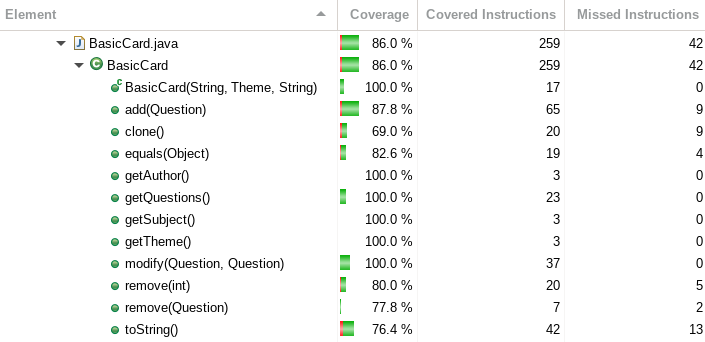
\includegraphics[width=\textwidth]{junit_coverage.png}
	\caption{Rapport de couverture du code}
	\label{fig:diag_coverage}
\end{figure}

